\section{Methodology}
For this study, literature review is conducted as a preliminary task. This process involved the searching of relevant research paper; for this purpose key words and phrases are used in famous repository including; ACM, IEEE, DBLP and Google Scholar. First the identified key-words are used, then their synonyms and other appropriate and applicable words used in found paper are searched to accomplish the collection of literature.The basic set of seed words are "content based recommendation system", "News recommendation", "textual recommendation", "user reviews recommendation", "document recommendation", "articles recommendation". In next phase of filtering, the papers which were based on ranking techniques or using other content such as video and images were omitted. 
To present the studies in an effective format, the articles from all the genres are highlighted, But as the focus of research has been shifted towards deep learning and latest work is inclined towards using it in one way or other. Due to this very reason this survey also discussed extensively the details about deep learning techniques used in recommendation systems. The survey compiles the work done during the time period of 2000-2019. A year wise distribution is presented in following graph.
\newline
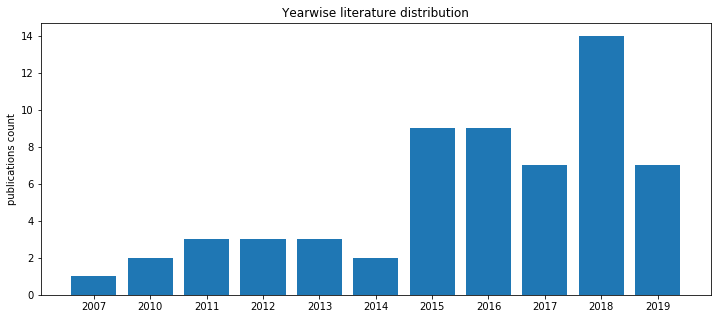
\includegraphics[width=12cm]{images/literaturedistribution.png}
\newline

The complete method to conduct this study is summarized in the figure shown below.After initial searches there is a huge number (270) of articles found. The acquired articles were then classified in major categorise. The categorization was done on the basis of their titles. The tentative count of these categorizes are mentioned.
\\1. Deep learning based
\\2. Knowledge graph based
\\3. Concept based
 After categorization of acquired literature; selected articles were studied in detail. The state-of the art approaches of feature selection, and algorithms were listed These articles were then  categorized into two types; metadata and key-insights. Later, state-of-the-art approaches and data-sets against each category were determined. After this whole process,all the research findings against this study are consolidated to present the current state in this domain. 
 \newline
 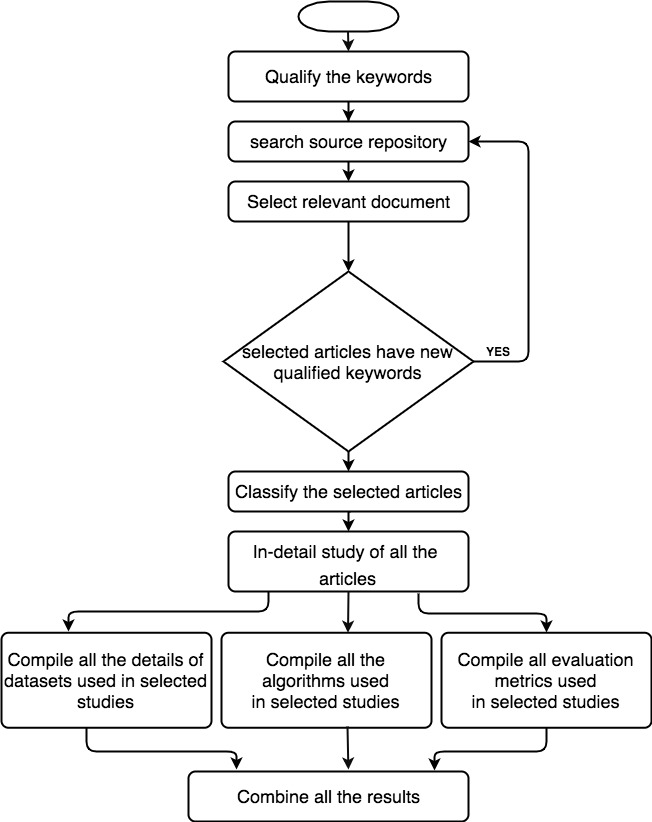
\includegraphics[width=14cm]{images/surveymethidilogy.jpg}
\pagebreak{}
